% !TEX program = pdflatex
% !TeX encoding = utf8
% !TeX spellcheck = pl-PL

%%%%%%%%%%%%%%%%%%%%%%%%%%%%%%%%%%%%%%%%%%%%%%%%%%%%%%%%%%%%%%%%%%%%%%%%%%%
% Wybierz rodzaj pracy dyplomowej oraz wydział
% Pick thesis type and faculty
%%%%%%%%%%%%%%%%%%%%%%%%%%%%%%%%%%%%%%%%%%%%%%%%%%%%%%%%%%%%%%%%%%%%%%%%%%%
\documentclass[thesis=inz,faculty=ee]{EE-dyplom} 

% thesis=[inz|mgr|bsc|msc]
%  * inz - praca inżynierska
%  * mgr - praca magisterska
%  * bsc - bachelor thesis
%  * msc - master thesis

% Skróty nazw wydziałów zgodne z domenami internetowymi
% Abbreviations of Faculties according to Internet subdomains
% faculty=[
%	arch,
%	gik,
%	ee,
%	wip
%	]

%%%%%%%%%%%%%%%%%%%%%%%%%%%%%%%%%%%%%%%%%%%%%%%%%%%%%%%%%%%%%%%%%%%%%%%%%%%
% Konfiguracja - do personalizacji
% Configuration - to be personalized
%%%%%%%%%%%%%%%%%%%%%%%%%%%%%%%%%%%%%%%%%%%%%%%%%%%%%%%%%%%%%%%%%%%%%%%%%%%
\instytut{Instytut Sterowania i Elektroniki Przemysłowej}
\kierunek{Automatyka i Robotyka Stosowana}
\title{Opracowanie oprogramowania sterującego i przeprowadzenie testów obciążnicy pasywnej}
\engtitle{Development of control software and execution of passive load bank tests}
\album{331772}
\author{Szymon Bzura}
\promotor{prof. dr hab. inż. Arkadiusz Kaszewski}
\date{2026}
\longdate{2026-11-06}

%%%%%%%%%%%%%%%%%%%%%%%%%%%%%%%%%%%%%%%%%%%%%%%%%%%%%%%%%%%%%%%%%%%%%%%%%%%
% Streszczenie pracy i abstract.
% In case of thesis in English swap the order - English version goes first.
%%%%%%%%%%%%%%%%%%%%%%%%%%%%%%%%%%%%%%%%%%%%%%%%%%%%%%%%%%%%%%%%%%%%%%%%%%%
\streszczeniepracy{
To jest streszczenie. To jest trochę za krótkie, jako że powinno zająć całą stronę.

Streszczenie to nie to samo co wstęp. Streszczenie przedstawia informacje o tym, co się znajduje w tekście poszczególnych rozdziałów danej pracy podczas gdy ,,Wstęp'' służy przedstawieniu zagadnienia podjętego w~pracy. Streszczenie prezentuje aktualny stan pracy dyplomowej, której pisanie zostało zakończone a~więc należy w~nim posługiwać się czasem teraźniejszym.

} % koniec streszczenia

\slowakluczowe{A, B, C}

\thesisabstract{
This is abstract. This one is a little too short as it should occupy the whole page.

An abstract is not the same as an introduction. The abstract provides information about what is contained in the text of specific chapters of a given work, whereas the introduction serves to present the topic addressed in the work. The abstract presents the current state of the diploma thesis, the writing of which has been completed, and therefore it should be written in the present tense.
} % end of abstract

\thesiskeywords{X, Y, Z}

%%%%%%%%%%%%%%%%%%%%%%%%%%%%%%%%%%%%%%%%%%%%%%%%%%%%%%%%%%%%%%%%%%%%%%%%%%%
% Tu zaczyna się dokument
% Here is the beginning of the document
%%%%%%%%%%%%%%%%%%%%%%%%%%%%%%%%%%%%%%%%%%%%%%%%%%%%%%%%%%%%%%%%%%%%%%%%%%%
\begin{document}
    % Strony nagłówkowe - musi być
    % Headers - must exist
    \frontpages
    
    % Tekst pracy - osobne pliki do edycji
    % Thesis text - separate files for edition

	% Tekst pracy - modułowy podział na rozdziały
	\chapter{Wstęp i cel pracy}
\label{chap:wstep}

\section{Wprowadzenie}
% Tutaj ogólny zarys problematyki (rola obciążnic w testowaniu zasilaczy i falowników).

\section{Cel i zakres pracy}
% Sformułowanie głównego celu inżynierskiego oraz wypunktowanie 6 zadań z zakresu.

\section{Struktura pracy}
% Krótki opis jednym zdaniem, co zawiera każdy z kolejnych rozdziałów.
	\chapter{Architektura sprzętowa i analiza dokumentacji technicznej}
\label{chap:analiza_sprzetu}

\section{Opis stanowiska badawczego}
% Wprowadzenie do zrealizowanej wcześniej części sprzętowej (PCB, obudowa).
Stanowisko badawcze ma formę autonomicznej, trójmodułowej obciążnicy pasywnej prądu stałego, umożliwiającej skokową regulację pobieranej mocy. Architektura fizyczna urządzenia została zaprojektowana z uwzględnieniem separacji obwodów silnoprądowych od układów cyfrowego sterowania. Cały system składa się z następujących głównych bloków:

\begin{itemize}
	\item \textbf{Tor główny:} Badane źródło zasilania podłączane jest za pomocą zacisków bananowych z lewej strony obudowy. Jest ono izolowane i zabezpieczane od reszty układu poprzez styczniki GIGAVAC.
	
	\item \textbf{Moduły wykonawcze:} Każdy z trzech modułów wyposażony jest we własny radiator z rezystorami mocy. Układ został wyposażony w wentylatory do chłodzenia powietrznego, zamontowane od dołu bloku rezystorów oraz termistory NTC do pomiaru temperatury. Uzupełnieniem chłodzenia całego systemu są dwa wentylatory umieszczone na górze obudowy.
	
	\item \textbf{Układ kondycjonowania sygnałów i przełączania:} Płyta przekaźników sterujących stanowi interfejs między mikrokontrolerem a torem mocy. Znajdują się na niej przetworniki prądu i napięcia umożliwiające akwizycję tych wielkości do postaci cyfrowej. Ponadto, płyta ta zawiera przekaźniki zmieniające konfigurację połączenia rezystorów mocy w celu zmiany obciążenia oraz dedykowany przekaźnik wysterowujący główne styczniki próżniowe GIGAVAC.
	
	\item \textbf{Jednostka centralna:} Algorytmy sterowania oraz maszyna stanów realizowane są przez główną płytę cyfrową, której sercem jest procesor sygnałowy Texas Instruments TMS320F28069.
	
	\item \textbf{Zasilanie pomocnicze:}  Energia niezbędna do zasilania elektroniki, cewek przekaźników oraz wentylatorów dostarczana jest z pokładowego zasilacza LRS-75-24, który zasilany jest z napięcia sieciowego zabezpieczonego bezpiecznikiem nadprądowym EATON o charakterystyce B6. Zasilacz znamionowo dostarcza napięcie 24V oraz prąd 3.2A
	
	\item \textbf{Lokalny interfejs użytkownika (HMI):} Panel przedni urządzenia umożliwia pracę stanowiska bez udziału komputera nadrzędnego. Wyposażono go w wyświetlacz alfanumeryczny, sygnalizacyjne diody LED oraz przełączniki dwu- i trójpozycyjne służące do ręcznego ustalania trybu pracy i konfiguracji obciążenia. Komunikację z systemami zewnętrznymi umożliwiają dwa porty DB9 których głównym zadaniem jest obsługa magistrali CAN. Panel przedni posiada również port USB-B służący do programowania mikrokontrolera.
\end{itemize}

Architekturę sprzętową stanowiska zilustrowano na schemacie blokowym (Rysunek \ref{fig:schemat_blokowy}).

% Tutaj wstawisz wygenerowany z Draw.io schemat blokowy
 \begin{figure}[htb]
	     \centering
	     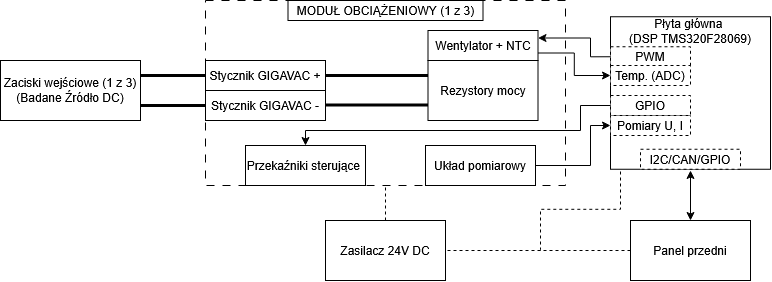
\includegraphics[width=\textwidth]{rysunki/schemat_blokowy_obciaznicy}
	     \caption{Schemat blokowy obciążnicy pasywnej z uwzględnieniem jednego modułu wykonawczego}
	     \label{fig:schemat_blokowy}
	 \end{figure}



\section{Mikrokontroler TMS320F28069}
% Analiza noty katalogowej rodziny C2000 i peryferiów użytych w projekcie (ADC, ePWM, eCAN).

\section{Moduły wykonawcze i styczniki GIGAVAC}
% Opis układu załączania obciążeń (rezystory 5.5/22/88 omów) i parametrów styczników.

\section{Układy pomiarowe i sensoryka}
% Pomiary napięć, prądów, czujniki NTC oraz izolacja galwaniczna układu.
	\chapter{Koncepcja i założenia oprogramowania sterującego}
\label{chap:zalozenia_fsm}

\section{Architektura systemu sterowania}
% Ogólny schemat blokowy oprogramowania wbudowanego i podział na zadania.

\section{Projekt maszyny stanów (FSM)}
% Graf przejść, opis głównych stanów (np. INIT, IDLE, RUN, FAULT) i warunków zmiany.

\section{Algorytm bezpiecznego przełączania (Break-before-make)}
% Założenia czasowe dla styczników, zabezpieczenie przed łukiem elektrycznym i zwarciami.

\section{Zabezpieczenia sprzętowe i programowe}
% Reakcja na przekroczenie prądu, temperatury oraz utratę komunikacji (timeout).
	\chapter{Implementacja oprogramowania wbudowanego mikrokontrolera}
\label{chap:firmware}

\section{Konfiguracja środowiska i peryferiów}
% Ustawienia w Code Composer Studio, inicjalizacja zegarów, GPIO i przerwań.

\section{Akwizycja i przetwarzanie sygnałów (ADC)}
% Konfiguracja pomiarów i skalowanie wartości z przetwornika na jednostki fizyczne (V, A).

\section{Realizacja maszyny stanów i sterowanie}
% Kod C odpowiedzialny za logikę FSM, włączanie GIGAVACów oraz sterowanie PWM chłodzeniem.

\section{Zarządzanie czasem i Watchdog}
% Krytyczne procedury czasowe, timery sprzętowe i zabezpieczenie przed zawieszeniem układu.
	\chapter{Interfejs telemetrii i zdalnego sterowania magistralą CAN}
\label{chap:telemetria}

\section{Warstwa fizyczna i konfiguracja kontrolera eCAN}
% Ustawienia bitrate (1 Mbps), parametry czasowe magistrali i izolacja.

\section{Struktura ramek danych}
% Opis ramek wysyłanych (telemetria: U, I, T, status FSM) i odbieranych (komendy sterujące).

\section{Mechanizmy weryfikacji i sprzężenia zwrotnego}
% Potwierdzanie wykonania komendy i programowe sprawdzanie rzeczywistego przepływu prądu.

\section{Lokalny interfejs użytkownika}
% Komunikacja I2C i prezentacja parametrów na lokalnym wyświetlaczu LCD.
	\chapter{Środowisko automatyzacji testów w programie MATLAB}
\label{chap:matlab}

\section{Integracja interfejsu PCAN-USB}
% Wykorzystanie bibliotek/Vehicle Network Toolbox do nawiązania komunikacji z PC.

\section{Akwizycja i parsowanie danych w czasie rzeczywistym}
% Odbiór telemetrii, rozkodowanie ramek i wizualizacja parametrów pomiarowych.

\section{Generowanie profili obciążeniowych (HIL)}
% Skrypty wymuszające dynamiczne sekwencje testowe i automatyczne sterowanie obciążnicą.

\section{Rejestracja wyników i raportowanie}
% Zapis logów do plików (np. CSV) i generowanie przebiegów z testów.
	\chapter{Instrukcja stanowiskowa i procedury bezpieczeństwa}
\label{chap:instrukcja}

\section{Zasady BHP przy pracy z urządzeniem}
% Środki ostrożności, ostrzeżenia o wysokich napięciach i temperaturach.

\section{Procedura podłączania badanych obiektów}
% Krok po kroku: jak prawidłowo podłączyć źródło zasilania (np. falownik) do terminali.

\section{Procedura uruchomienia i obsługi}
% Kolejność włączania zasilania, start aplikacji w MATLABie, tryb ręczny vs automatyczny.

\section{Sytuacje awaryjne i rozwiązywanie problemów}
% Co robić w przypadku wejścia w stan FAULT, przegrzania lub błędu magistrali CAN.
	\chapter{Podsumowanie i wnioski}
\label{chap:podsumowanie}

\section{Ocena realizacji celów pracy}
% Zestawienie osiągniętych funkcjonalności z założeniami opisanymi we wstępie.

\section{Wnioski z przeprowadzonych testów}
% Krótkie omówienie poprawności działania środowiska HIL i stabilności sprzętu.

\section{Perspektywy dalszego rozwoju}
% Co można ulepszyć w przyszłości (np. nowy interfejs webowy, szybsze algorytmy).

    % Bibliografia - musi być, jest w pliku EE-dyplom.bib
    % Bibliography - must exist, is in the file EE-dyplom.bib
    \bibliografia

    % Strony końcowe - można zakomentować, jeśli zbędne
    % Additional pages - comment out if not needed
    
    % Wykaz symboli i skrótów - patrz opis w tekście przykładowym
    \acronymslist
    % Spis rysunków
    \listoffigures
    % Spis tabel
    \listoftables
    % Załączniki (plik appendices.tex)
    %\easyappendices
\end{document}
%%%%%%%%%%%%%%%%%%%%%%%%%%%%%%%%%%%%%%%%%%%%%%%%%%%%%%%%%%%%%%%%%%%%%%%%%%%

